\chapter{User Interface Overview}

\section{Interactive Elements}
\subsection{Axes}
While most axes in the GUI are non-interactive, you can use the options in the upper-right corner for basic interactions. For advanced interaction, use the \textit{Tool $\rightarrow$ Pop-out Figure Menu Bar} to open the figure in MATLAB. (See Section~\ref{sec:menu})
\begin{figure}[H]
    \centering
    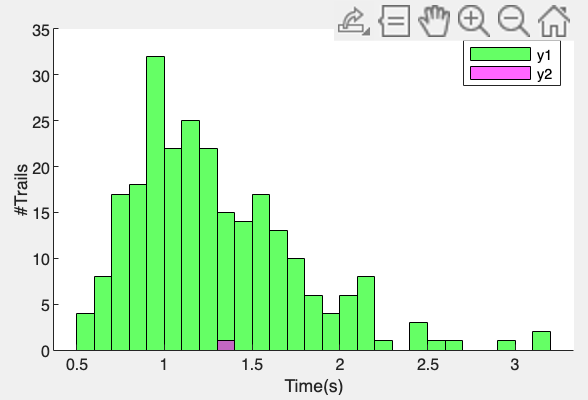
\includegraphics[width=0.5\textwidth]{figs/axes_image.png}
    \caption{Axes Interaction Example.}
    \label{fig:axes}
\end{figure}

\subsection{Button}
Press a button to execute the associated action.
\begin{figure}[H]
    \centering
    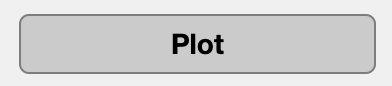
\includegraphics[width=0.35\textwidth]{figs/button_image.png}
    \caption{Example of a Button.}
    \label{fig:button}
\end{figure}

\subsection{Check Box}
Toggle the check box to enable or disable specific features.
\begin{figure}[H]
    \centering
    
\includegraphics[width=0.25\textwidth]{figs/checkbox_image.png}
    \caption{Example of a Check Box.}
    \label{fig:checkbox}
\end{figure}

\subsection{Drop Down}
Select an option by clicking the drop-down menu.
\begin{figure}[H]
    \centering
    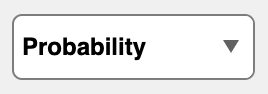
\includegraphics[width=0.25\textwidth]{figs/dropdown_image.png}
    \caption{Drop-down Menu Example.}
    \label{fig:dropdown}
\end{figure}

\subsection{Edit Field (Numeric)}
Enter a single numeric value within the specified range.
\begin{figure}[H]
    \centering
    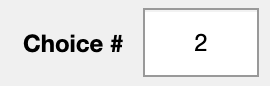
\includegraphics[width=0.25\textwidth]{figs/edit_field_image.png}
    \caption{Numeric Edit Field Example.}
    \label{fig:edit_field}
\end{figure}

\subsection{Menu Bar}\label{sec:menu}
The GUI features three main menu options: File, Tools, and Help. Note that not all submenus are available in every window.
\begin{itemize}
	\item \textbf{File}:
	\begin{itemize}
	\item Import existing simulation data or batch files
	\item Export figures to a specified directory
	\end{itemize}
	\item \textbf{Tools}:
	\begin{itemize}
		\item Batch file generator
		\item Pop-out figures for separate viewing
		\item Axis customization:
		\begin{itemize}
			\item X-axis: Toggle between $W_s$ and Tau display
			\item Y-axis: Switch between linear and logarithmic scales
		\end{itemize}
		\item Data smoothing options
	\end{itemize}

	\item \textbf{Help}:
	\begin{itemize}
		\item Link to this documentation
	\end{itemize}
\end{itemize}

\subsection{Slider}
Move the slider to adjust its value. For values outside the slider’s range, enter them directly into the associated numeric field.
\begin{figure}[H]
    \centering
    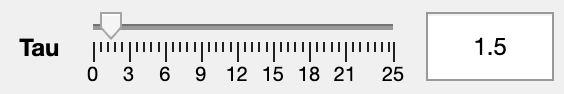
\includegraphics[width=0.55\textwidth]{figs/slider_image.png}
    \caption{Slider Example.}
    \label{fig:slider}
\end{figure}

\subsection{Text Area}\label{sec:text_area}
Provide input based on the displayed instructions. You may enter multiple values in the text area, separated by commas. Alternatively, you can use a specific convention for entering values, such as:
\begin{itemize}
    \item \( \text{zeros(1,20)} \) for a row vector of 20 zeros,
    \item \( \text{ones(3,4)} \) for a 3x4 matrix of ones,
    \item \( 1:20:100 \) for a sequence from 1 to 100 with a step size of 20.
\end{itemize}

These conventions allow for more flexible input formats that the system can interpret.

\begin{figure}[H]
    \centering
    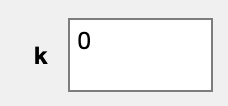
\includegraphics[width=0.2\textwidth]{figs/text_area_image.png}
    \caption{Interactive Text Area Example.}
    \label{fig:text_area}
\end{figure}

\subsection{Tree (Check Box)}
Check or uncheck nodes to customize selections.
\begin{figure}[H]
    \centering
    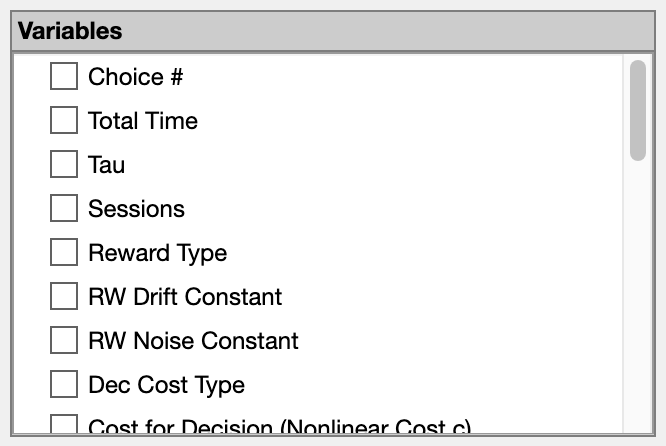
\includegraphics[width=0.55\textwidth]{figs/tree_checkbox_image.png}
    \caption{Tree with Check Boxes Example.}
    \label{fig:tree_checkbox}
\end{figure}

\section{Noninteractive Elements}
\subsection{Progress Gauge (Linear)}
Displays the progress of the current simulation.
\begin{figure}[H]
    \centering
    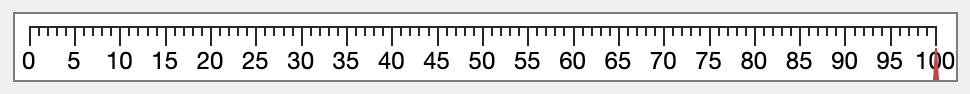
\includegraphics[width=0.7\textwidth]{figs/progress_gauge_image.png}
    \caption{Linear Progress Gauge Example.}
    \label{fig:progress_gauge}
\end{figure}

\subsection{Lamp} \label{sec:status_lamp}
Indicates simulation status:
\begin{itemize}
    \item \textbf{Gray:} Idle state.
    \item \textbf{Green:} Simulation in progress.
    \item \textbf{Red:} Error.
\end{itemize}
\begin{figure}[H]
    \centering
    
\includegraphics[width=0.25\textwidth]{figs/lamp_image_grey.png}
    \caption{Lamp Indicator Example.}
    \label{fig:lamp}
\end{figure}

\subsection{Text Area}
Displays read-only information such as block time, settings summaries, or total rewards.
\begin{figure}[H]
    \centering
    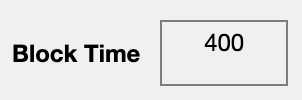
\includegraphics[width=0.25\textwidth]{figs/noninteractive_text_area_image.png}
    \caption{Non-interactive Text Area Example.}
    \label{fig:noninteractive_text_area}
\end{figure}